%%%%%%%%%%%%%%%%%%%%%%%%%%%%%%%%%%%%%%%%%%%%%%%%%%%%%%%%%%%%%%%%%%%%%%%%%%%%%%%%%%
%%																				%%
%% File name: 		21hannes.tex												%%
%% Project name:	Hochleistungsantenne										%%
%% Type of work:	T3X00 project work											%%
%% Author:			Sarah Brückner, Maximilian Stiefel, Hannes Bohnengel		%%
%% Date:			01st May 2016												%%
%% University:		DHBW Ravensburg Campus Friedrichshafen						%%
%% Comments:		Created in gedit with tab width = 4							%%
%%																				%%
%%%%%%%%%%%%%%%%%%%%%%%%%%%%%%%%%%%%%%%%%%%%%%%%%%%%%%%%%%%%%%%%%%%%%%%%%%%%%%%%%%

\chapter{GPredict}

\section{Übersicht}




\cite{gpredictsource}

\section{Grafische Oberfläche}

\begin{itemize}
	\parskip0pt
	\item Radio Control
	\item Rotator Control
    \item Sky at a Glance
    \item Time Controller
    \item Modul-Einstellungen (Configure)
    \item Polar View
    \item Single Sat View (Pass Details)
\end{itemize}

\clearpage

\begin{figure}[h]
	\centering
	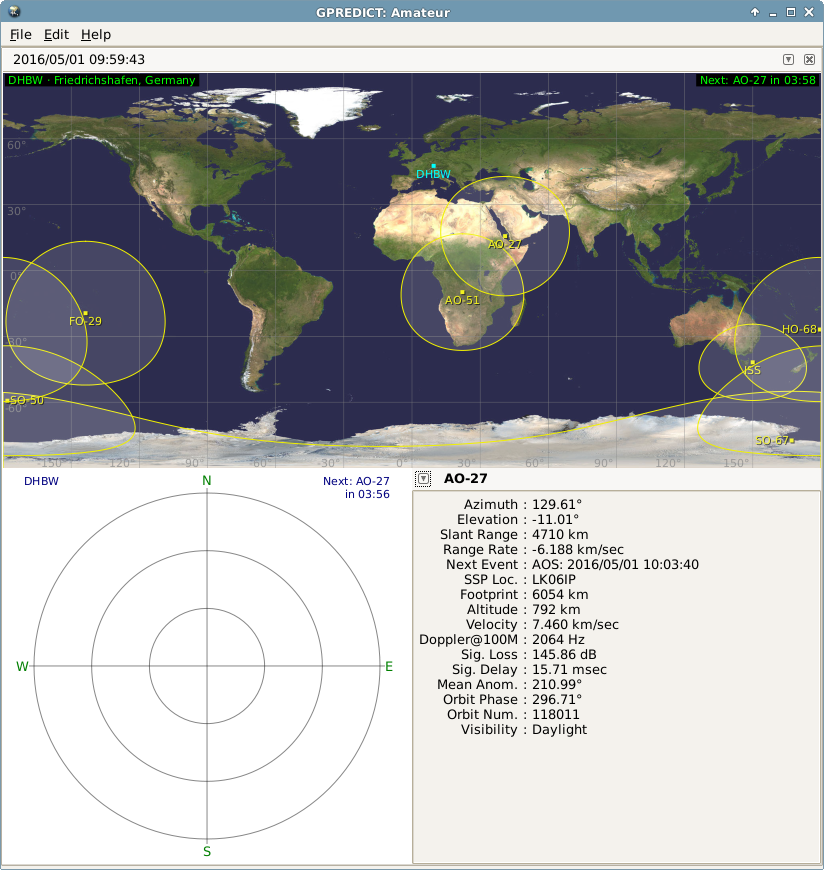
\includegraphics[width=0.8\textwidth]{gpredict-startup.png}
	\caption[Standardoberfläche von GPredict]{Standardoberfläche von GPredict}
	\label{fig:gpredict-startup} 
\end{figure}

\section{Inbetriebnahme unter Windows}

\section{Inbetriebnahme unter Linux}